\chapter{Diagrams}
\label{appendix:d}

  \begin{figure}[h!]
    \centering
    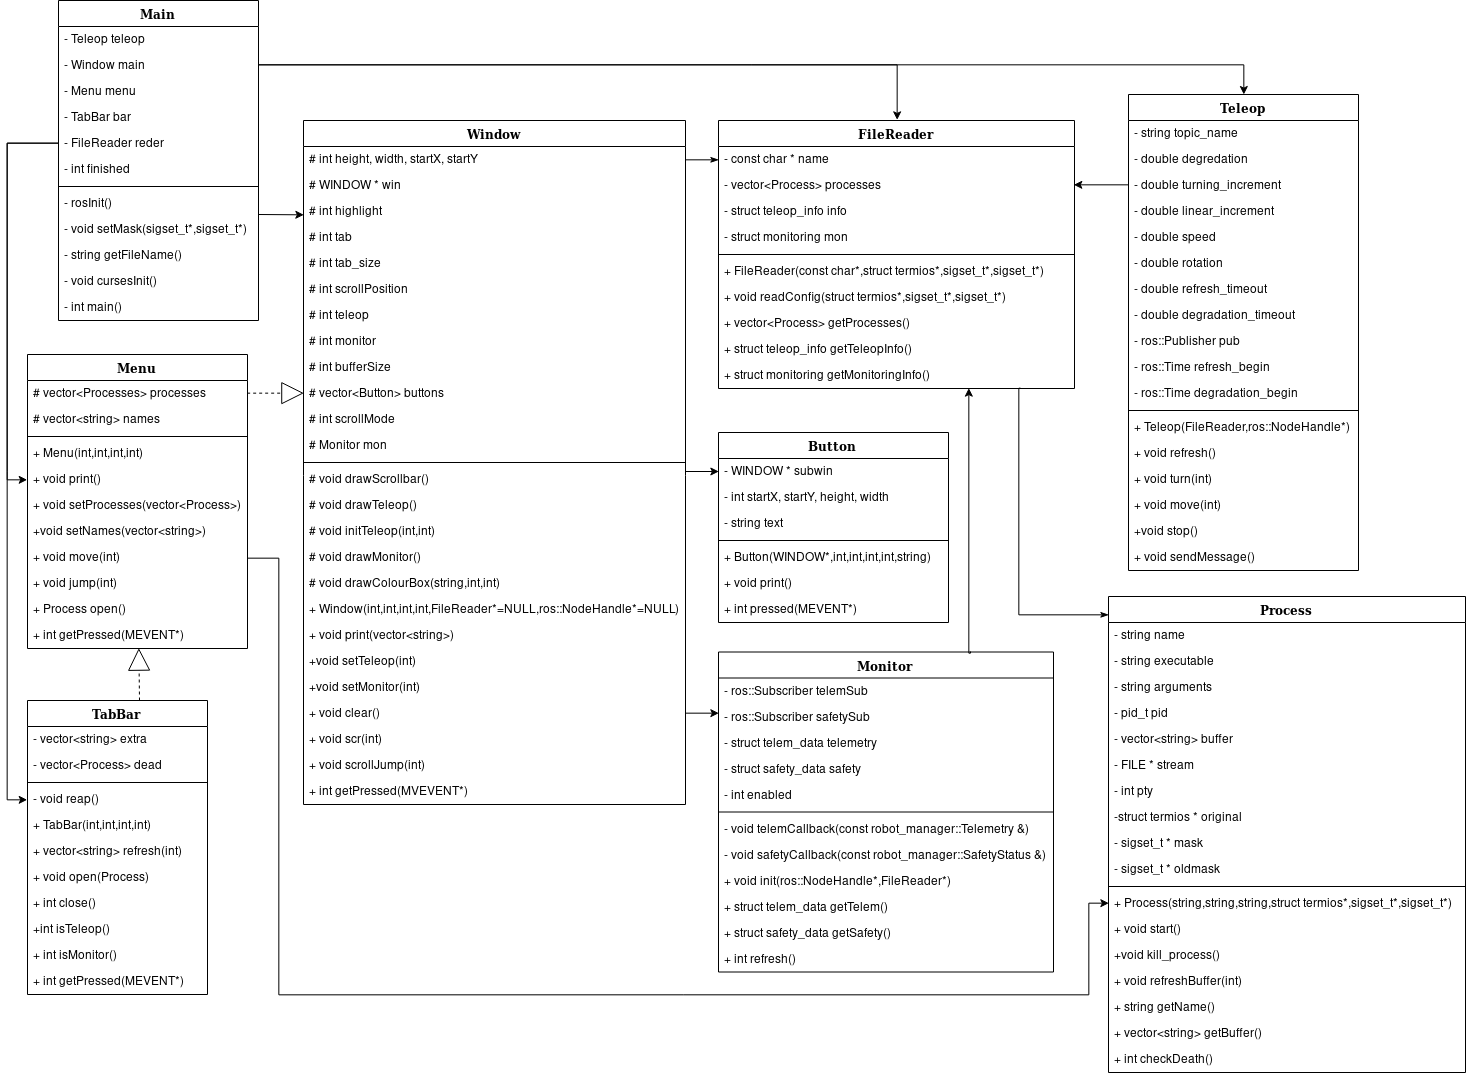
\includegraphics[scale=0.43,angle=-90]{ClassDiagramNew}
    \caption{UML class diagram of the final system}
    \label{fig:class-diagram}
  \end{figure}

  \begin{figure}[h!]
    \centering
    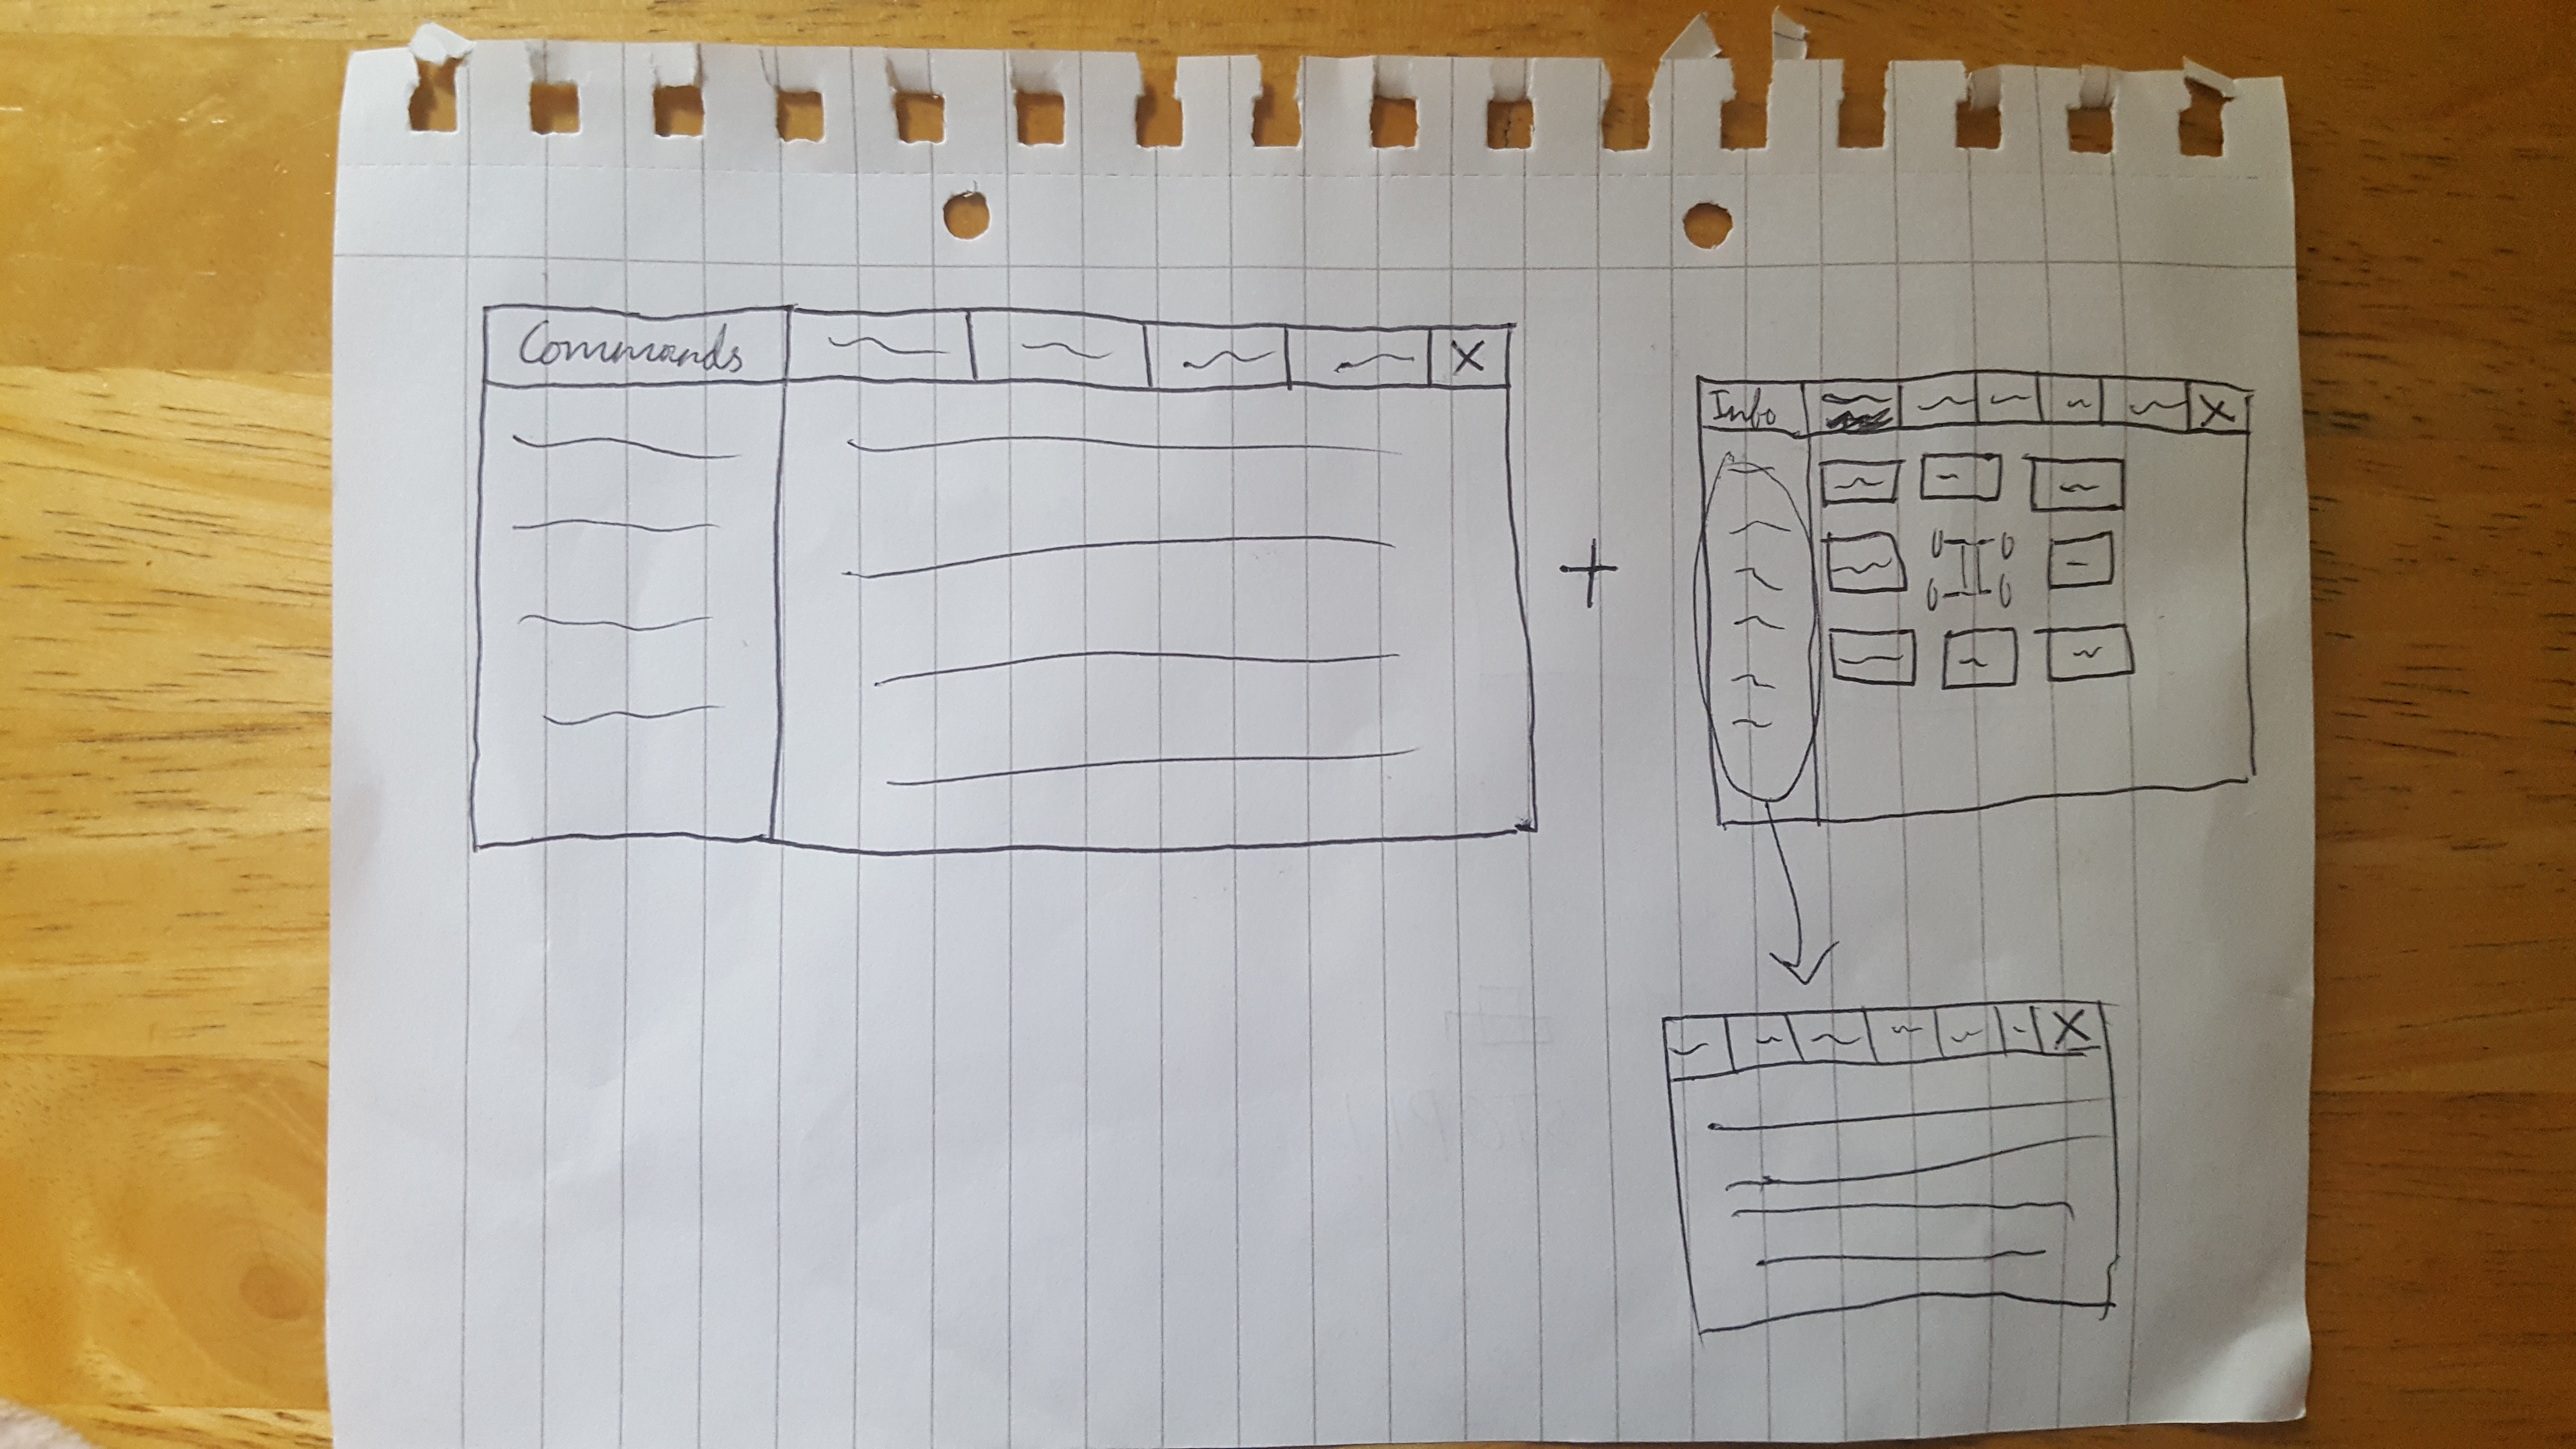
\includegraphics[scale=0.08]{UISketch01}
    \caption{Initial drawing of what the user interface was planned to look like}
    \label{fig:sketch01}
  \end{figure}

  \begin{figure}[h!]
    \centering
    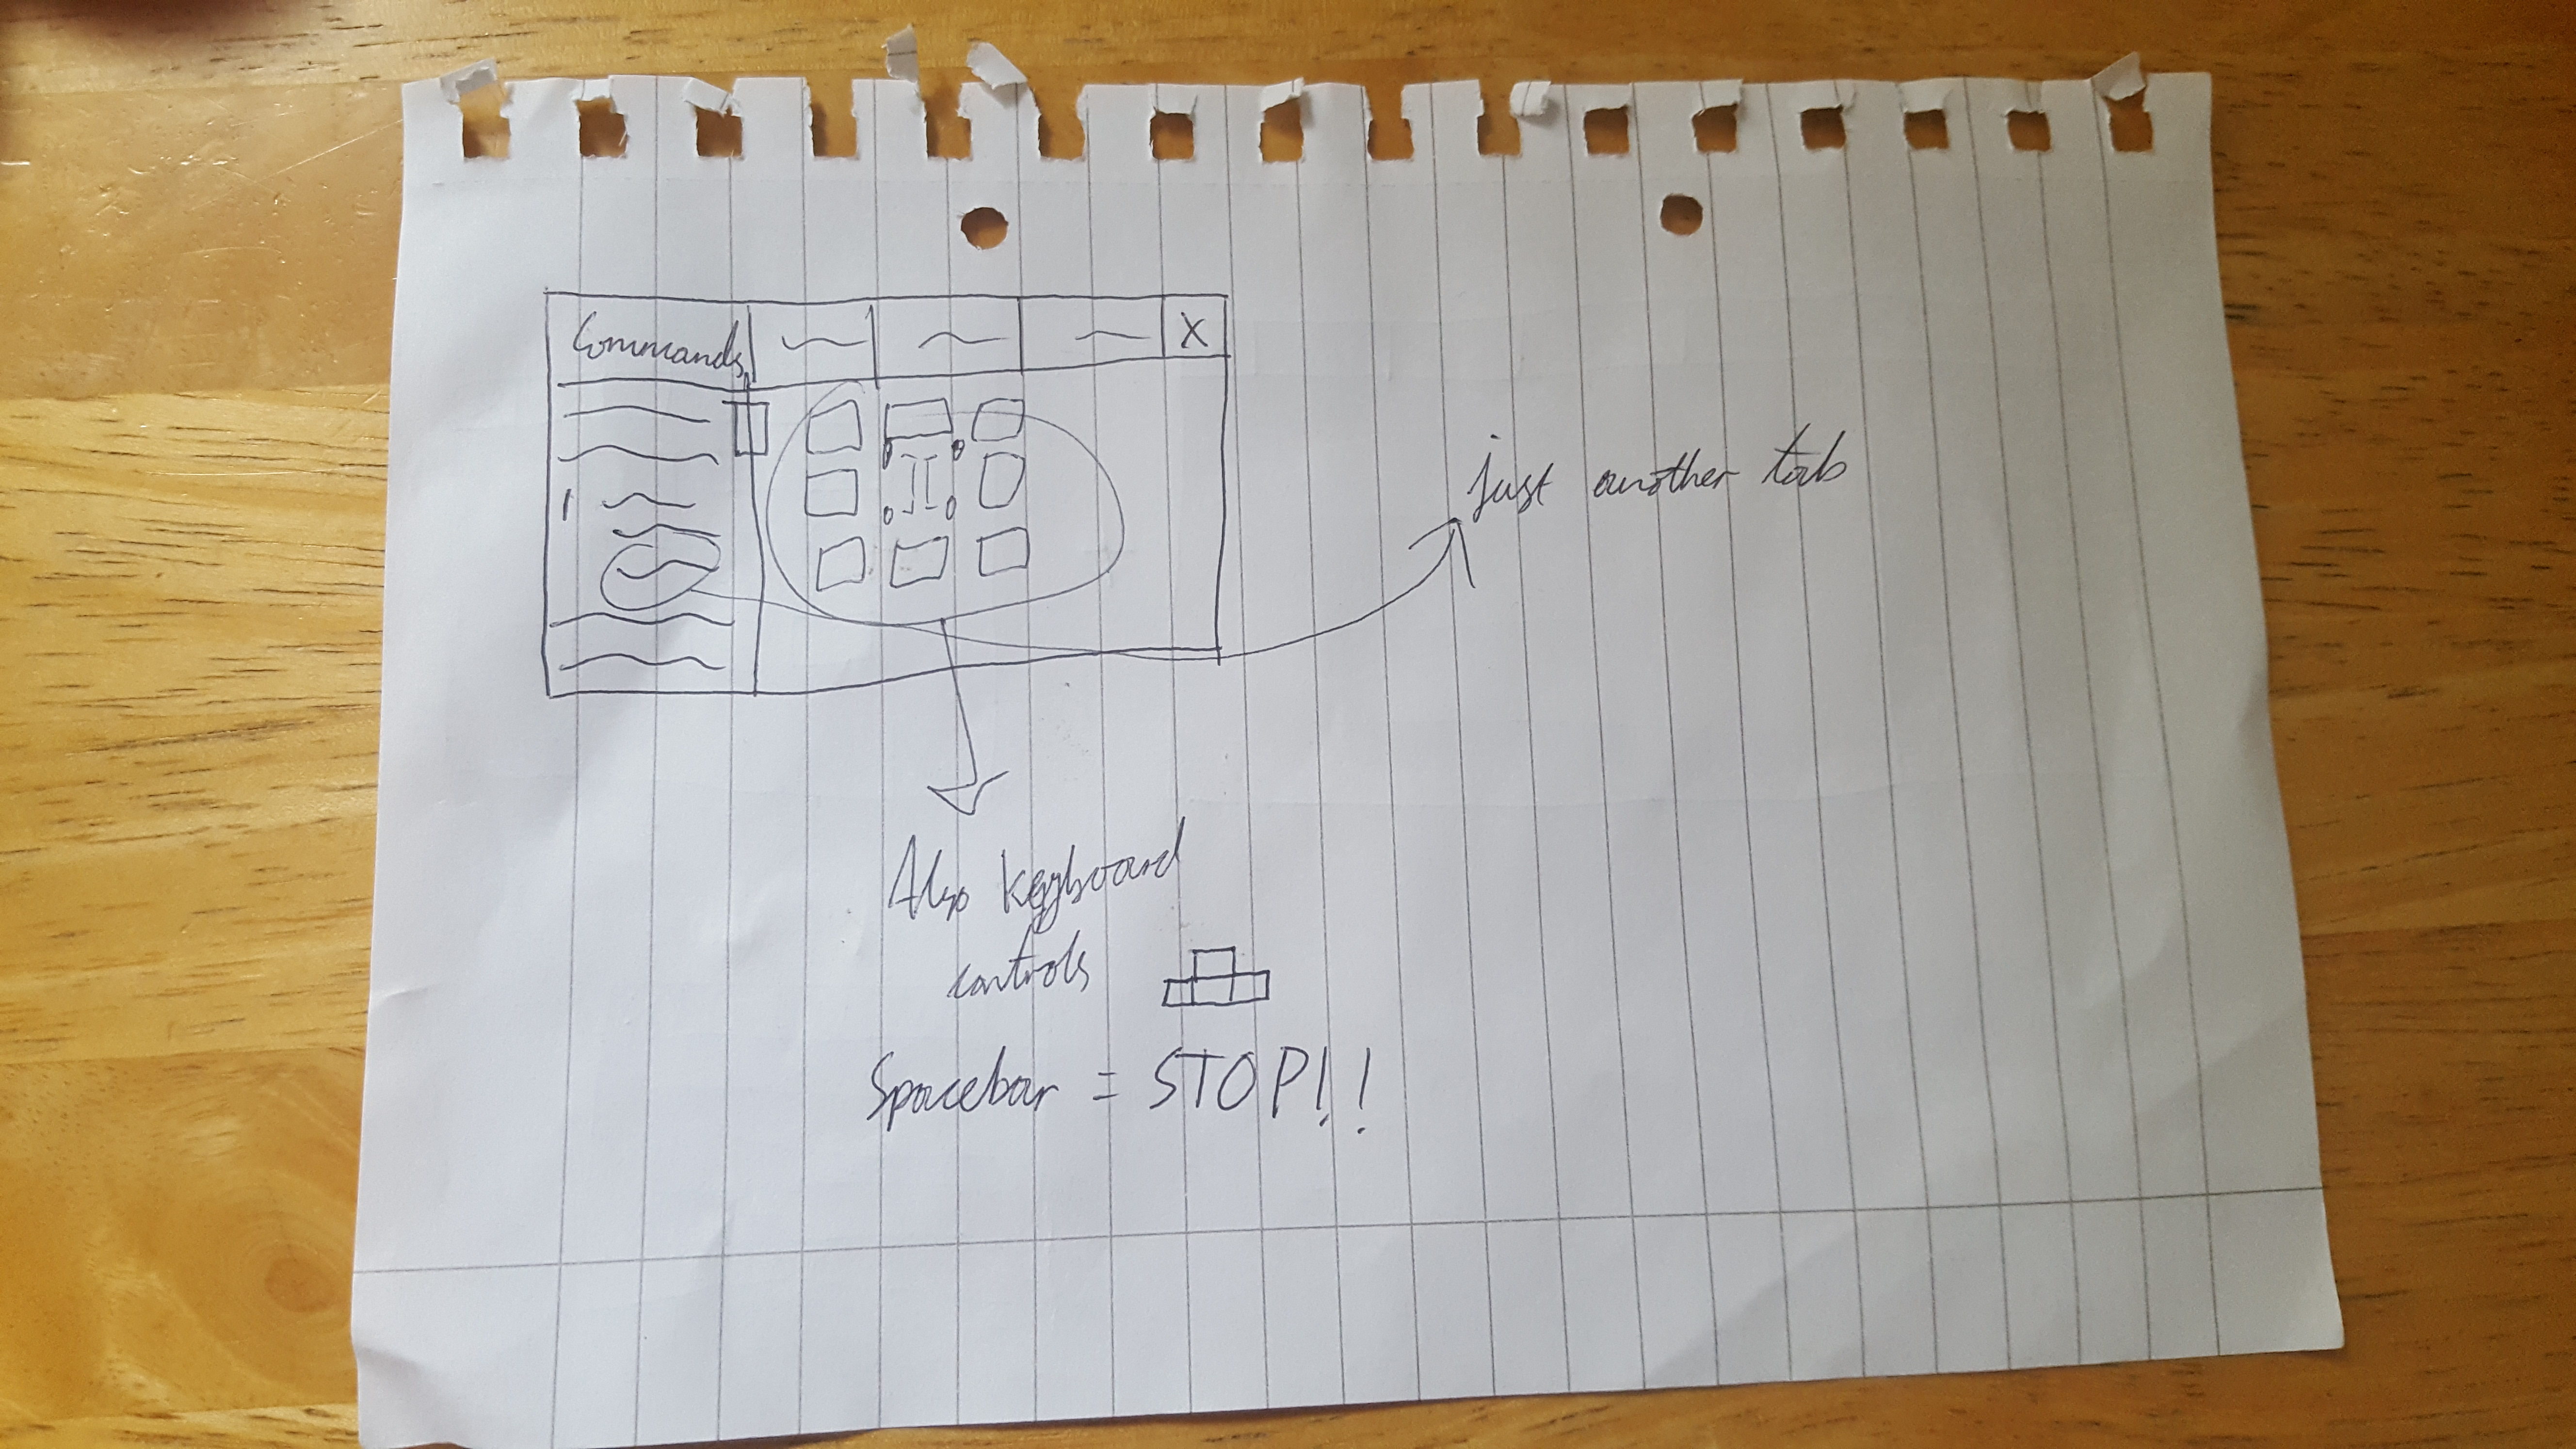
\includegraphics[scale=0.08]{UISketch02}
    \caption{Altered design to account for changes in client requirements and to have as much as possible on one screen}
    \label{fig:sketch02}
  \end{figure}
